
\section{Issues and Motivations}
\label{sec:motivations}

Causal broadcast is a communication primitive that allows a process to send
messages to all processes of its distributed system (\REF). Message deliveries
follow the happen before relationship (\REF). If the sending of a message $m$
precedes the sending of a message $m'$ then all processes that deliver these two
messages need to deliver $m$ before $m'$. Otherwise they deliver them in any
order. Each process may receive a message multiple times but it delivers it
exactly once.

Causal broadcast has properties about reliability. First, it guarantees that all
correct processes eventually receive broadcast messages. Gossiping constitutes
an efficient mean to reliably disseminate messages to large systems (\REF). Each
process maintains a partial view considerably smaller than the whole system
membership. When a process broadcasts a message, it sends it to its partial
view; each process that receives such message forwards it to its partial
view. Broadcast messages reach all processes either directly or transitively.

\begin{figure*}
  \begin{center}
    \subfloat[Part A][\label{fig:generalpurgeA}Process~A broadcasts $a$. It expects 
    two copies of the message $a$.]
    {
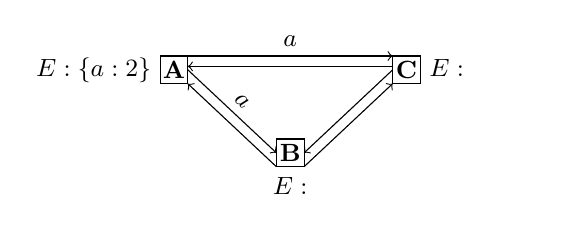
\begin{tikzpicture}[scale=1]
  
  \small
  
  \newcommand\X{210/5pt};
  \newcommand\Y{30pt};
  
  % \draw[->] ( -0.5*\X, 0.5*\Y) -- ( -5+0*\X, 0*\Y);
  % \draw[->] ( -0.5*\X, 0*\Y) -- ( -5+0*\X, 0*\Y);
  % \draw[->] ( -0.5*\X, -0.5*\Y) -- ( -5+0*\X, 0*\Y);  

  \draw[fill=white] (0*\X, 0*\Y) node{\textbf{A}} +(-5pt, -5pt) rectangle +(5pt, 5pt);
  \draw (-5+0*\X, 0*\Y) node[left]{$E: \{a:2\}$};
  \draw[fill=white] (1*\X, -1*\Y) node{\textbf{B}} +(-5pt, -5pt) rectangle +(5pt, 5pt);
  \draw (1*\X, -5-1*\Y) node[below]{$E: \varnothing$\vphantom{$\{$}};
  \draw[fill=white] (2*\X,  0*\Y) node{\textbf{C}} +(-5pt, -5pt) rectangle +(5pt, 5pt);
  \draw (5+2*\X, 0*\Y) node[right]{$E: \varnothing$\vphantom{$\{$}};
  \draw (5+2*\X, 0*\Y) node[right]{\phantom{$E: \{a:1\}$}};

  \draw[->](5+0*\X, 0*\Y) -- node[sloped, above]{$a$} (-5+1*\X, -1*\Y); %% A->B
  \draw[<-](5+0*\X, -5+0*\Y) -- (-5+1*\X, -5-1*\Y); %% A<-B

  \draw[->](5+0*\X, 5+0*\Y) -- node[above]{$a$} (-5+2*\X, 5+0*\Y); % A->C
  \draw[<-](5+0*\X,  1.25+ 0*\Y) -- (-5+2*\X,  1.25+ 0*\Y); % A<-C
 
  \draw[<-](5+1*\X, -1*\Y) -- (-5+2*\X, 0*\Y); %% B<-C
  \draw[->](5+1*\X, -5-1*\Y) -- (-5+2*\X, -5+0*\Y); %% B->C

  % \draw[->](5+2*\X, 0*\Y) -- ( 2.5*\X, 0*\Y);
\end{tikzpicture}}
    \hspace{10pt}
    \subfloat[Part B][\label{fig:generalpurgeB}Process~B and Process~C receive
    and deliver $a$. Process~C expected an additional copy of the message $a$
    while Process~B does not.]
    {
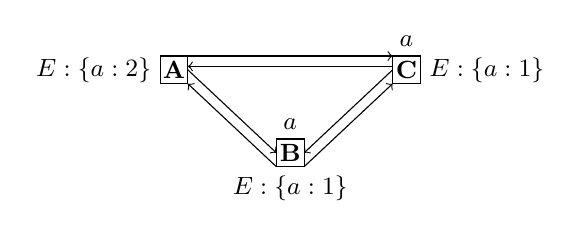
\begin{tikzpicture}[scale=1]
  
  \small
  
  \newcommand\X{210/5pt};
  \newcommand\Y{30pt};
  
  % \draw[->] ( -0.5*\X, 0.5*\Y) -- ( -5+0*\X, 0*\Y);
  % \draw[->] ( -0.5*\X, 0*\Y) -- ( -5+0*\X, 0*\Y);
  % \draw[->] ( -0.5*\X, -0.5*\Y) -- ( -5+0*\X, 0*\Y);  

  \draw[fill=white] (0*\X, 0*\Y) node{\textbf{A}} +(-5pt, -5pt) rectangle +(5pt, 5pt);
  \draw (-5+0*\X, 0*\Y) node[left]{$E: \{a:2\}$};
  \draw[fill=white] (1*\X, -1*\Y) node{\textbf{B}} +(-5pt, -5pt) rectangle +(5pt, 5pt);
  \draw (1*\X, 5-1*\Y) node[above]{$a$};
  \draw (1*\X, -5-1*\Y) node[below]{$E:\{a:1\}$};
  \draw[fill=white] (2*\X,  0*\Y) node{\textbf{C}} +(-5pt, -5pt) rectangle +(5pt, 5pt);
  \draw (2*\X, 5-0*\Y) node[above]{$a$};
  \draw (5+2*\X, 0*\Y) node[right]{$E:\{a:1\}$};

  \draw[->](5+0*\X, 0*\Y) -- (-5+1*\X, -1*\Y); %% A->B
  \draw[<-](5+0*\X, -5+0*\Y) -- (-5+1*\X, -5-1*\Y); %% A<-B

  \draw[->](5+0*\X, 5+0*\Y) -- (-5+2*\X, 5+0*\Y); % A->C
  \draw[<-](5+0*\X,  1.25+ 0*\Y) -- (-5+2*\X,  1.25+ 0*\Y); % A<-C
 
  \draw[<-](5+1*\X, -1*\Y) -- (-5+2*\X, 0*\Y); %% B<-C
  \draw[->](5+1*\X, -5-1*\Y) -- (-5+2*\X, -5+0*\Y); %% B->C

  % \draw[->](5+2*\X, 0*\Y) -- ( 2.5*\X, 0*\Y);
\end{tikzpicture}}
    \hspace{10pt}
    \subfloat[Part C][\label{fig:generalpurgeC}Process~B and Process~C forward $a$ 
    to their neighbors in a gossip fashion.]
    {
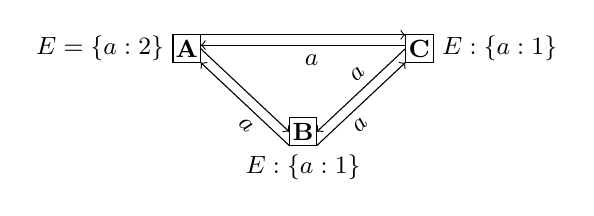
\begin{tikzpicture}[scale=1]
  
  \small
  
  \newcommand\X{210/5pt};
  \newcommand\Y{30pt};
  
  \draw[fill=white] (0*\X, 0*\Y) node{\textbf{A}} +(-5pt, -5pt) rectangle +(5pt, 5pt);
  \draw (-5+0*\X, 0*\Y) node[left]{$E = \{a:2\}$};
  \draw[fill=white] (1*\X, -1*\Y) node{\textbf{B}} +(-5pt, -5pt) rectangle +(5pt, 5pt);
%  \draw (1*\X, 5-1*\Y) node[above]{$a$};
  \draw (1*\X, -5-1*\Y) node[below]{$E:\{a:1\}$};
  \draw[fill=white] (2*\X,  0*\Y) node{\textbf{C}} +(-5pt, -5pt) rectangle +(5pt, 5pt);
%  \draw (2*\X, 5-0*\Y) node[above]{$a$};
  \draw (5+2*\X, 0*\Y) node[right]{$E:\{a:1\}$};

  \draw[->](5+0*\X, 0*\Y) -- (-5+1*\X, -1*\Y); %% A->B
  \draw[<-](5+0*\X, -5+0*\Y) -- node[sloped, below]{$\,\,\,\,\,\,\,a$} (-5+1*\X, -5-1*\Y); %% A<-B

  \draw[->](5+0*\X, 5+0*\Y) -- (-5+2*\X, 5+0*\Y); % A->C
  \draw[<-](5+0*\X,  1.25+ 0*\Y) -- node[below]{$\,\,\,\,a$} (-5+2*\X,  1.25+ 0*\Y); % A<-C
 
  \draw[<-](5+1*\X, -1*\Y) -- node[sloped,above]{$\,\,\,\,a$} (-5+2*\X, 0*\Y); %% B<-C
  \draw[->](5+1*\X, -5-1*\Y) -- node[sloped,below]{$a\,\,\,\,\,\,\,$}(-5+2*\X, -5+0*\Y); %% B->C

  % \draw[->](5+2*\X, 0*\Y) -- ( 2.5*\X, 0*\Y);
\end{tikzpicture}}
    \hspace{10pt}
    \subfloat[Part D][\label{fig:generalpurgeD}Process~A and Process~C receive a copy
    of $a$. Process~C does not expect additional copies of the message $a$. 
    Process~A still expects a copy.]
    {
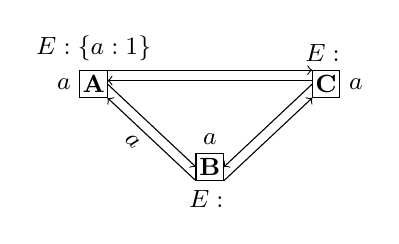
\begin{tikzpicture}[scale=1]
  
  \small
  
  \newcommand\X{210/5pt};
  \newcommand\Y{30pt};
  
  \draw[fill=white] (0*\X, 0*\Y) node{\textbf{A}} +(-5pt, -5pt) rectangle +(5pt, 5pt);
  \draw (-5+0*\X, 0*\Y) node[left]{$a$};
  \draw (0*\X, 5+0*\Y) node[above]{$E: \{a:\bm{1}\}$};
  \draw[fill=white] (1*\X, -1*\Y) node{\textbf{B}} +(-5pt, -5pt) rectangle +(5pt, 5pt);
  \draw (1*\X, 5-1*\Y) node[above]{$a$};
  \draw (1*\X, -5-1*\Y) node[below]{$E:\bm{\varnothing}$};%\vphantom{$\{$}};
  \draw[fill=white] (2*\X,  0*\Y) node{\textbf{C}} +(-5pt, -5pt) rectangle +(5pt, 5pt);
  \draw (5+2*\X, 0*\Y) node[right]{$a$};
  \draw (2*\X, 5+0*\Y) node[above]{$E:\bm{\varnothing}$};%\vphantom{$\{$}};
%  \draw (5+2*\X, 0*\Y) node[right]{\phantom{$E:\{a:1\}$}};

  \draw[->](5+0*\X, 0*\Y) -- (-5+1*\X, -1*\Y); %% A->B
  \draw[<-](5+0*\X, -5+0*\Y) -- node[sloped, below]{$a\,\,\,\,\,\,$} (-5+1*\X, -5-1*\Y); %% A<-B

  \draw[->](5+0*\X, 5+0*\Y) -- (-5+2*\X, 5+0*\Y); % A->C
  \draw[<-](5+0*\X,  1.25+ 0*\Y) -- (-5+2*\X,  1.25+ 0*\Y); % A<-C
 
  \draw[<-](5+1*\X, -1*\Y) -- (-5+2*\X, 0*\Y); %% B<-C
  \draw[->](5+1*\X, -5-1*\Y) -- (-5+2*\X, -5+0*\Y); %% B->C

  % \draw[->](5+2*\X, 0*\Y) -- ( 2.5*\X, 0*\Y);
\end{tikzpicture}}
    \hspace{10pt}
    \subfloat[Part E][\label{fig:generalpurgeE}Process~A receives the last 
    awaited copy of the message $a$. It purges its structure from this message.]
    {
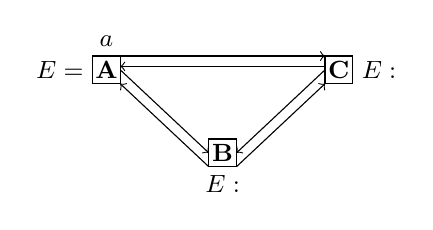
\begin{tikzpicture}[scale=1]
  
  \small
  
  \newcommand\X{210/5pt};
  \newcommand\Y{30pt};
  
  \draw[fill=white] (0*\X, 0*\Y) node{\textbf{A}} +(-5pt, -5pt) rectangle +(5pt, 5pt);
  \draw (0*\X, 5-0*\Y) node[above]{$a$};
  \draw (-5+0*\X, 0*\Y) node[left]{$E = \varnothing$};
  \draw[fill=white] (1*\X, -1*\Y) node{\textbf{B}} +(-5pt, -5pt) rectangle +(5pt, 5pt);
  \draw (1*\X, -5-1*\Y) node[below]{$E:\varnothing$};
  \draw[fill=white] (2*\X,  0*\Y) node{\textbf{C}} +(-5pt, -5pt) rectangle +(5pt, 5pt);
  \draw (5+2*\X, 0*\Y) node[right]{$E:\varnothing$};

  \draw[->](5+0*\X, 0*\Y) -- (-5+1*\X, -1*\Y); %% A->B
  \draw[<-](5+0*\X, -5+0*\Y) -- (-5+1*\X, -5-1*\Y); %% A<-B

  \draw[->](5+0*\X, 5+0*\Y) -- (-5+2*\X, 5+0*\Y); % A->C
  \draw[<-](5+0*\X,  1.25+ 0*\Y) -- (-5+2*\X,  1.25+ 0*\Y); % A<-C
 
  \draw[<-](5+1*\X, -1*\Y) -- (-5+2*\X, 0*\Y); %% B<-C
  \draw[->](5+1*\X, -5-1*\Y) -- (-5+2*\X, -5+0*\Y); %% B->C

  % \draw[->](5+2*\X, 0*\Y) -- ( 2.5*\X, 0*\Y);
\end{tikzpicture}}
    \caption{\label{fig:generalpurge}Broadcast that guarantees to deliver 
      messages exactly once using counters.}
  \end{center}
\end{figure*}


\begin{algorithm}
  \SetKwProg{Function}{function}{}{}
\SetKwProg{Upon}{upon}{}{}
\SetKwProg{Initially}{INITIALLY:}{}{}
\SetKwProg{Dissemination}{DISSEMINATION:}{}{}

\small

\DontPrintSemicolon
\LinesNumbered

\Initially {} {
  $Q_o$ \tcp*{Set of processes, $p$'s outview}
  $Q_i$ \tcp*{Set of processes, $p$'s inview}
  \BlankLine
  $E \leftarrow \varnothing$ \tcp*{message $\rightarrow$  \# of expected copies}
}

\BlankLine

\Dissemination{}{
  
  \Function{$\textup{R-broadcast}(m)$} { %\tcp*[f]{$b_p(m)$}} { 
    % $\textup{received}(m,\, \_)$ \;
    % lForEach {$q \in Q_o$} {\textup{sendTo}($q,\, m$)}
    % \textup{R-deliver}($m$) \; % \tcp*{$d_p(m)$}
    $\textup{receive}(m,\, \_)$ \;
  }

  \BlankLine
  
  \Upon{$\textup{receive}(m,\, l)$}{
    \If {$\neg\textup{received}(m,\,l)$} {
      \lForEach {$q \in Q_o$} {\textup{sendTo}($q,\, m$) \tcp*[f]{fwd}}
      \textup{R-deliver}($m$) \; % \tcp*{$d_p(m)$}
    }
  }

  \BlankLine
  
  \Function{$\textup{received}(m,\, l)$}{
    \textbf{let} $hasReceived \leftarrow m \in E$ \;
    \lIf { $\neg hasReceived$ } { $E[m] \leftarrow |Q_i|$ \tcp*[f]{init}}
    \lIf { $l\not\in Q_i$} {$E[m] \leftarrow E[m] - 1$ \tcp*[f]{count}} 
    \lIf { $E[m] = 0$ } { $E \leftarrow E\setminus m$ \tcp*[f]{purge}}
    \Return $hasReceived$ \;
  }
  
}


%%% Local Variables:
%%% mode: latex
%%% TeX-master: "../paper"
%%% End:

  \caption{\label{algo:counterrbroadcast}R-broadcast at Process $p$ using
    temporary counters.}
\end{algorithm}


Second, it guarantees that each process delivers each broadcast message exactly
once, in spite of multiple receipts that can occur.
Figure~\ref{fig:generalpurge} shows a scenario involving 3 processes using the
lightweight implementation of reliable broadcast in
Algorithm~\ref{algo:counterrbroadcast}.  The idea consists in recording the
number of copies expected after the first receipt. When the expected number of
copies falls to zero, the process will never receive this message
again. Consequently, it safely purges its local structure from this element. In
Figure~\ref{fig:generalpurgeA}, Process~A broadcasts $a$ to Process~B and
Process~C. Since it knows that each process forwards each message exactly once,
it expects to receive 2 copies: one from Process~B, one from Process~C. In
Figure~\ref{fig:generalpurgeB}, Process~B and Process~C receive and deliver
$a$. Process~B does not expect copies of this message. Process~C expects an
additional copy of this message from Process~B.  Since this is their first
receipt of $a$, Process~B and Process~C deliver and forward $a$ to their
neighbors. In Figure~\ref{fig:generalpurgeD}, Process~C receives the awaited
copy of $a$. It will never receive such message again, so it removes it from its
set of expected messages $E$. Process~A receives a copy but does not purge its
local structure, for it still expect an additional copy of the message. It
decrements the counter corresponding to $a$. In Figure~\ref{fig:generalpurgeE},
Process~A finally receives the last copy of $a$ and purges its structure.

\begin{figure*}
  \begin{center}
    \subfloat[Part A][\label{fig:generalproblemA}Process~A broadcasts $a$.]
    {
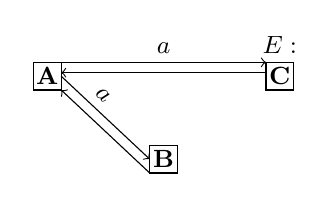
\begin{tikzpicture}[scale=1]
  
  \small
  
  \newcommand\X{210/5pt};
  \newcommand\Y{30pt};

  
  \draw[fill=white] (0*\X, 0*\Y) node{\textbf{A}} +(-5pt, -5pt) rectangle +(5pt, 5pt);
  % \draw (-5+0*\X, 0*\Y) node[left]{$E: \{a:2\}$};
  \draw[fill=white] (1*\X, -1*\Y) node{\textbf{B}} +(-5pt, -5pt) rectangle +(5pt, 5pt);
  % \draw (1*\X, -5-1*\Y) node[below]{$E: \varnothing$\vphantom{$\{$}};
  \draw[fill=white] (2*\X,  0*\Y) node{\textbf{C}} +(-5pt, -5pt) rectangle +(5pt, 5pt);
  \draw (2*\X, 5+0*\Y) node[above]{$E: \varnothing$};%%$\vphantom{$\{$}};
  % \draw (5+2*\X, 0*\Y) node[right]{\phantom{$E: \{a:1\}$}};
  
  \draw[->](5+0*\X, 0*\Y) -- node[sloped,above]{$\bm{a}$~~~~~} (-5+1*\X, -1*\Y); %% A->B
  \draw[<-](5+0*\X, -5+0*\Y) -- (-5+1*\X, -5-1*\Y); %% A<-B
  
  \draw[->](5+0*\X, 5+0*\Y) -- node[above]{$\bm{a}$} (-5+2*\X, 5+0*\Y); % A->C
  \draw[<-](5+0*\X,  1.25+ 0*\Y) -- (-5+2*\X,  1.25+ 0*\Y); % A<-C
  
  % \draw[->,dashed](5+1*\X, -1*\Y) -- (-5+2*\X, 0*\Y); %% B<-C
  % \draw[->, dashed](5+1*\X, -5-1*\Y) -- (-5+2*\X, -5+0*\Y); %% B->C



\end{tikzpicture}}
    \hspace{10pt}
    \subfloat[Part B][\label{fig:generalproblemB}Process~C receives,
    delivers, and forwards $a$. It does not expect additional copies.]
    {
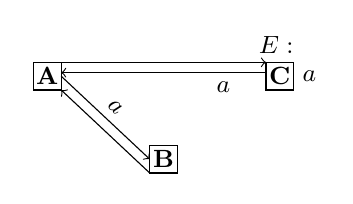
\begin{tikzpicture}[scale=1]
  
  \small
  
  \newcommand\X{210/5pt};
  \newcommand\Y{30pt};

  
  \draw[fill=white] (0*\X, 0*\Y) node{\textbf{A}} +(-5pt, -5pt) rectangle +(5pt, 5pt);
  % \draw (-5+0*\X, 0*\Y) node[left]{$E: \{a:2\}$};
  \draw[fill=white] (1*\X, -1*\Y) node{\textbf{B}} +(-5pt, -5pt) rectangle +(5pt, 5pt);
  % \draw (1*\X, -5-1*\Y) node[below]{$E: \varnothing$\vphantom{$\{$}};
  \draw[fill=white] (2*\X,  0*\Y) node{\textbf{C}} +(-5pt, -5pt) rectangle +(5pt, 5pt);
  \draw (2*\X, 5+0*\Y) node[above]{$E: \bm{\varnothing}$};%%$\vphantom{$\{$}};
  \draw (5+2*\X, 0*\Y) node[right]{$\bm{a}$};
  
  \draw[->](5+0*\X, 0*\Y) -- node[sloped,above]{$a$} (-5+1*\X, -1*\Y); %% A->B
  \draw[<-](5+0*\X, -5+0*\Y) -- (-5+1*\X, -5-1*\Y); %% A<-B
  
  \draw[->](5+0*\X, 5+0*\Y) -- (-5+2*\X, 5+0*\Y); % A->C
  \draw[<-](5+0*\X,  1.25+ 0*\Y) -- node[below]{~~~~~~~~~~~~~~$a$} (-5+2*\X,  1.25+ 0*\Y); % A<-C
  
  % \draw[->,dashed](5+1*\X, -1*\Y) -- (-5+2*\X, 0*\Y); %% B<-C
  % \draw[->, dashed](5+1*\X, -5-1*\Y) -- (-5+2*\X, -5+0*\Y); %% B->C



\end{tikzpicture}}
    \hspace{10pt}
    \subfloat[Part C][\label{fig:generalproblemC}Process~B adds Process~C as neighbor.]
    {
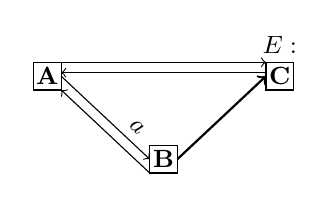
\begin{tikzpicture}[scale=1]
  
  \small
  
  \newcommand\X{210/5pt};
  \newcommand\Y{30pt};

  
  \draw[fill=white] (0*\X, 0*\Y) node{\textbf{A}} +(-5pt, -5pt) rectangle +(5pt, 5pt);
  % \draw (-5+0*\X, 0*\Y) node[left]{$E: \{a:2\}$};
  \draw[fill=white] (1*\X, -1*\Y) node{\textbf{B}} +(-5pt, -5pt) rectangle +(5pt, 5pt);
  % \draw (1*\X, -5-1*\Y) node[below]{$E: \varnothing$\vphantom{$\{$}};
  \draw[fill=white] (2*\X,  0*\Y) node{\textbf{C}} +(-5pt, -5pt) rectangle +(5pt, 5pt);
  \draw (2*\X, 5+0*\Y) node[above]{$E: \varnothing$};%%$\vphantom{$\{$}};
  % \draw (5+2*\X, 0*\Y) node[right]{\phantom{$E: \{a:1\}$}};
  
  \draw[->](5+0*\X, 0*\Y) -- node[sloped,above]{~~~~~~~$a$} (-5+1*\X, -1*\Y); %% A->B
  \draw[<-](5+0*\X, -5+0*\Y) -- (-5+1*\X, -5-1*\Y); %% A<-B
  
  \draw[->](5+0*\X, 5+0*\Y) -- (-5+2*\X, 5+0*\Y); % A->C
  \draw[<-](5+0*\X,  1.25+ 0*\Y) -- (-5+2*\X,  1.25+ 0*\Y); % A<-C
  
  \draw[->,thick](5+1*\X, -1*\Y) -- (-5+2*\X, 0*\Y); %% B<-C
  % \draw[->, dashed](5+1*\X, -5-1*\Y) -- (-5+2*\X, -5+0*\Y); %% B->C



\end{tikzpicture}}    
    \hspace{10pt}
    \subfloat[Part D][\label{fig:generalproblemD}Process~B receives, delivers,
    and forwards $a$. Among others, it sends a copy of $a$ to Process~C.]
    {
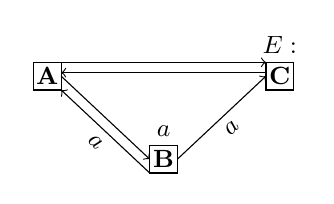
\begin{tikzpicture}[scale=1]
  
  \small
  
  \newcommand\X{210/5pt};
  \newcommand\Y{30pt};

  
  \draw[fill=white] (0*\X, 0*\Y) node{\textbf{A}} +(-5pt, -5pt) rectangle +(5pt, 5pt);
  % \draw (-5+0*\X, 0*\Y) node[left]{$E: \{a:2\}$};
  \draw[fill=white] (1*\X, -1*\Y) node{\textbf{B}} +(-5pt, -5pt) rectangle +(5pt, 5pt);
  \draw (1*\X, 5-1*\Y) node[above]{$\bm{a}$};
  \draw[fill=white] (2*\X,  0*\Y) node{\textbf{C}} +(-5pt, -5pt) rectangle +(5pt, 5pt);
  \draw (2*\X, 5+0*\Y) node[above]{$E: \varnothing$};%%$\vphantom{$\{$}};
  % \draw (5+2*\X, 0*\Y) node[right]{\phantom{$E: \{a:1\}$}};
  
  \draw[->](5+0*\X, 0*\Y) -- (-5+1*\X, -1*\Y); %% A->B
  \draw[<-](5+0*\X, -5+0*\Y) -- node[sloped,below]{$a$} (-5+1*\X, -5-1*\Y); %% A<-B
  
  \draw[->](5+0*\X, 5+0*\Y) -- (-5+2*\X, 5+0*\Y); % A->C
  \draw[<-](5+0*\X,  1.25+ 0*\Y) -- (-5+2*\X,  1.25+ 0*\Y); % A<-C
  
  \draw[->](5+1*\X, -1*\Y) -- node[below, sloped]{$\bm{a}$}(-5+2*\X, 0*\Y); %% B<-C
  % \draw[->, dashed](5+1*\X, -5-1*\Y) -- (-5+2*\X, -5+0*\Y); %% B->C



\end{tikzpicture}}    
    \hspace{10pt}
    \subfloat[Part E][\label{fig:generalproblemE}Not only Process~C receives, delivers, 
    and forwards $a$ a second time, but it has cascading effects in the network.
    The expected number of copies becomes inconsistent and may grow unbounded.]
    {
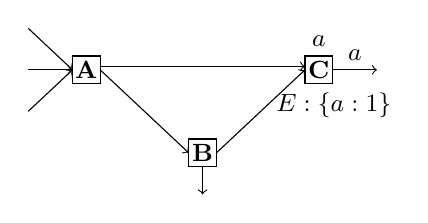
\begin{tikzpicture}[scale=1]
  
  \small
  
  \newcommand\X{210/5pt};
  \newcommand\Y{30pt};
  
  \draw[->] ( -0.5*\X, 0.5*\Y) -- ( -5+0*\X, 0*\Y);
  \draw[->] ( -0.5*\X, 0*\Y) -- ( -5+0*\X, 0*\Y);
  \draw[->] ( -0.5*\X, -0.5*\Y) -- ( -5+0*\X, 0*\Y);  

%  \draw[->] ( 5+2*\X, 0*\Y) -- ( 2.5*\X, 0.5*\Y);
  \draw[->] ( 5+2*\X, 0*\Y) -- node[above]{$a$} ( 2.5*\X, 0*\Y);
%  \draw[->] ( 5+2*\X, 0*\Y) -- ( 2.5*\X, -0.5*\Y);  

%  \draw[->] ( 1*\X, -5-1*\Y) -- ( 1.5*\X, -1.5*\Y);
  \draw[->] ( 1*\X, -5-1*\Y) -- ( 1*\X, -1.5*\Y);
%  \draw[->] ( 1*\X, -5-1*\Y) -- ( 0.5*\X, -1.5*\Y);  


  \draw[fill=white] (0*\X, 0*\Y) node{\textbf{A}} +(-5pt, -5pt) rectangle +(5pt, 5pt);
%  \draw (-5+0*\X, 0*\Y) node[left]{$E: \{a:2\}$};
  \draw[fill=white] (1*\X, -1*\Y) node{\textbf{B}} +(-5pt, -5pt) rectangle +(5pt, 5pt);
  % \draw (1*\X, 5-1*\Y) node[above]{$a$};
  \draw[fill=white] (2*\X,  0*\Y) node{\textbf{C}} +(-5pt, -5pt) rectangle +(5pt, 5pt);
  \draw (2*\X, 5-0*\Y) node[above]{$a$};
  \draw (2*\X, -5+0*\Y) node[below]{$\,\,\,\,\,\,\,E: \{a: 1\}$};
%%  \draw (5+2*\X, 0*\Y) node[right]{\phantom{$E: \{a:1\}$}};

  \draw[->](5+0*\X, 0*\Y) -- (-5+1*\X, -1*\Y); %% A->B

  \draw[->](5+0*\X,  1.25+ 0*\Y) -- (-5+2*\X,  1.25+ 0*\Y); % A->C
 
  \draw[->](5+1*\X, -1*\Y) -- (-5+2*\X, 0*\Y); %% B->C

\end{tikzpicture}}    
    \caption{\label{fig:generalproblem}In dynamic systems, the reliable
      broadcast using counters may deliver messages multiple times leading to
      inconsistencies.}
  \end{center}
\end{figure*}


Unfortunately, such implementation does not handle dynamic systems where
processes can join, leave, or self-reconfigure their partial view at any
time. Figure~\ref{fig:generalproblem} illustrates one of the issues. In
Figure~\ref{fig:generalproblemA}, Process~A broadcasts $a$. It sends a copy of
$a$ to its neighbors Process~B and Process~C. In
Figure~\ref{fig:generalproblemB}, Process~C receives $a$ for the first time.  As
consequence, it delivers and forwards it. Since Process~C has only 1 link
towards it, it does not expect additional copies of $a$. In
Figure~\ref{fig:generalproblemC}, Process~B adds Process~C as neighbors. In
Figure~\ref{fig:generalproblemD}, Process~B receives, delivers, and forwards
$a$. Since it added Process~C in its neighborhood, Process~B sends it a copy.
In Figure~\ref{fig:generalproblemE}, Process~C receives $a$ again. Since it did
not keep traces of its former receipt, Process~C believes that it receives $a$
for the first time. Process~C delivers, and forwards $a$ again. In addition, the
number of expected copies changes inconsistently. Processes may deliver messages
multiple times. Messages may travel through the system forever.

Even if this implementation does not work in dynamic systems, it gives the hint
that broadcast can guarantee reliability locally without maintaining costly data
structures summarizing the global state of the system, e.g., using vector
clocks.


% To solve this issue, state-of-the-art protocols maintain a local vector the size
% of which increases linearly with the number of processes that ever broadcast a
% message. They eventually become overcostly in dynamic settings.


In this paper, we exploit and extend \PCBROADCAST to provide a causal broadcast
middleware that is lightweight in terms of local memory consumption, and message
overhead. Table~\ref{table:complexity} shows its complexity. It keeps constant
message overhead and constant delivery execution time while removing the linear
dependency $N$ from the local space complexity. Its overhead in terms of number
of control messages is twice that of \PCBROADCAST.
%% It maintains a local structure that grows and shrinks over time when
%% processes can join, leave, or self-reconfigure their neighborhood over time.
%% \TODO{maybe more details.}
The next section describes the proposed protocol.

%%% Local Variables:
%%% mode: latex
%%% TeX-master: "../paper.tex"
%%% End:
